\documentclass[11pt]{article}

\usepackage[preprint]{acl}

\usepackage{times}
\usepackage{latexsym}
\usepackage[T1]{fontenc}
\usepackage[utf8]{inputenc}
\usepackage{microtype}
\usepackage{graphicx}
\usepackage{booktabs}
\usepackage{multirow}
\usepackage{amsmath}
\usepackage{xcolor}
\usepackage{tikz}
\usetikzlibrary{positioning,arrows.meta,fit}
\usepackage{pgfplots}
\pgfplotsset{compat=1.17}

\newcommand{\TBD}[1]{\textcolor{red}{[#1]}}
\newcommand{\savyar}{\textsc{Savyar}}
\newcommand{\gl}[1]{\textsc{#1}}
\newcommand{\tr}[1]{\textit{#1}}
\newcommand{\tok}[1]{\texttt{#1}}

\title{Root-Agnostic Morphological Disambiguation for Turkish}

\author{Anonymous \\
  Anonymous Affiliation \\
  \texttt{anonymous@example.org}}

\begin{document}
\maketitle

\begin{abstract}
A Turkish word form often has several morphological analyses, and the right one depends on the sentence. Neural disambiguators for Turkish represent each candidate analysis with its root, the surface word, or both. We present \savyar{}, a disambiguator that ranks the analyses of a rule-based analyzer without seeing any open-class root. Each word is reduced to a part-of-speech token for its root, or to one of 102 lexeme tokens for closed-class words, followed by its sequence of suffixes. A Transformer encodes every analysis, pools the analyses of each word, reads the words of the sentence together and chooses one analysis per word in a single pass. Because the ranker never sees the root, an unambiguous training word can be given the analyses of an ambiguous word whose gold analysis has the same encoding; this synthetic ambiguity adds 0.45 points on ambiguous words without new annotation. On TrMor2018, under the five-split protocol of \citet{akyurek-etal-2019-morphological}, \savyar{} reaches 96.16\% accuracy on all words and 92.05\% on ambiguous words. The analyzer proposes the gold analysis for 99.53\% of words, and sentence context adds 3.34 points over scoring each word alone. We report where the root abstraction fails and what these failures say about the division of labour between analyzer and ranker.
\end{abstract}

\section{Introduction}
\label{sec:introduction}

Turkish builds words by attaching suffixes to a root, and one surface form can result from different roots and different suffix sequences. A rule-based analyzer returns every analysis a word form admits \citep{oflazer-1994-two,ozturel-etal-2019-syntactically}. The word \tr{masalı} has three \citep{akyurek-etal-2019-morphological}:

\begin{center}
\small
\begin{tabular}{@{}lll@{}}
(1) a. & \tr{masa-lı} & table-\gl{with} `with a table' \\
\phantom{(1)} b. & \tr{masal-ı} & tale-\gl{acc} `the tale (object)' \\
\phantom{(1)} c. & \tr{masal-ı} & tale-\gl{poss.3sg} `his or her tale' \\
\end{tabular}
\end{center}

\noindent Only the sentence decides between them. \tr{Masalı yaz} `write the tale' needs (1b), \tr{babamın masalı} `my father's tale' needs (1c), and \tr{mavi masalı oda} `the room with a blue table' needs (1a). Morphological disambiguation is the task of choosing the analysis that fits the context \citep{hakkani-tur-etal-2018-morphological}.

Work on Turkish has moved from hand-written rules to statistical and neural models. Decision lists \citep{yuret-ture-2006-learning} and a perceptron reranker \citep{sak-etal-2007-morphological} reach 95.82\% and 96.28\% token accuracy on the hand-tagged TrMor2006 test set \citep{akyurek-etal-2019-morphological}. Neural disambiguators score each candidate analysis against a representation of its context \citep{yildiz-etal-2016-morphology,shen-etal-2016-role,toleu-etal-2017-character}. Sequence-to-sequence models drop the analyzer and generate the lemma and tags from characters \citep{akyurek-etal-2019-morphological,ozer-korkmaz-2022-transmorph}. On TrMor2018 the strongest of these reaches 98.59\% when it rescores the candidates of an analyzer instead of generating its own \citep{akyurek-etal-2019-morphological}.

All of these systems see the root. \citet{yildiz-etal-2016-morphology} embed it directly and gain about one point from pre-trained root embeddings. \citet{shen-etal-2016-role} read its characters, and generative models spell it out. The root carries lexical preferences, but in Turkish it also carries information that an analyzer can apply before any ranking takes place: which allomorph of the causative or of the aorist a verb takes, whether a stem loses its last vowel before a suffix, and which pronouns accept a possessive. Once these constraints are enforced during candidate generation, the remaining choice is often between suffix sequences: accusative or possessive, participle or finite verb, nominal or verbal reading of the stem. We ask how far a ranker gets on this choice when it sees only the suffix sequences of the whole sentence.

\savyar{} answers this with a strict division of labour. A rule-based analyzer generates the candidates and holds every rule that depends on the identity of the root. The ranker receives each word as a part-of-speech token for its root, or as a lexeme token for one of 102 closed-class words, followed by its suffixes. To the ranker, \tr{elma} `apple' and \tr{armut} `pear' are the same token. A Transformer encoder \citep{vaswani-etal-2017-attention} reads every analysis of every word in the sentence and chooses one analysis per word. Because roots are hidden, the only analysis of an unambiguous word such as \tr{kapıyı} `the door (\gl{acc})' has the same encoding as one analysis of an ambiguous word such as \tr{kitabı} `the book (\gl{acc})' or `his or her book'. Given the analyses of \tr{kitabı}, \tr{kapıyı} becomes an ambiguous training example whose label is known.

Our contributions are the following.
\begin{itemize}
\item A rule-based Turkish analyzer with 99 suffix types and a lexicon derived from a dictionary without reference to any treebank, in which root-dependent allomorphy is resolved before ranking (\S\ref{sec:analyzer}).
\item A root-agnostic ranker that chooses the analysis of each word given all analyses of the sentence (\S\ref{sec:ranker}), and synthetic ambiguity, a training scheme that the root abstraction makes possible (\S\ref{sec:training}).
\item An evaluation on TrMor2018 under the protocol of \citet{akyurek-etal-2019-morphological} that separates analyzer coverage from ranking accuracy and measures the contribution of sentence context (\S\ref{sec:results} and \S\ref{sec:analysis}).
\end{itemize}

\noindent Code, adapters and trained models will be released with the camera-ready version.

\section{Related Work}
\label{sec:related}

\paragraph{Analyzers.}
\citet{oflazer-1994-two} gave the first two-level description of Turkish morphology, with about 23,000 roots and 22 two-level rules. Its output format, a root followed by inflectional groups separated by derivational boundaries, is the annotation of the METU-Sabancı treebank \citep{oflazer-etal-2003-building} and of the TrMor data sets \citep{yuret-ture-2006-learning,akyurek-etal-2019-morphological}. \citet{ozturel-etal-2019-syntactically} released an open-source analyzer built with OpenFst, with 47,202 hand-annotated root entries, 51 inflectional and 72 derivational morphemes. It covers 95.56\% of the word types in the CoNLL 2007 Turkish data and returns 12.82 analyses per word form. Its feature scheme is the annotation of the Turkish Web Treebank \citep{kayadelen-etal-2020-gold}.

\paragraph{Disambiguation over analyzer output.}
\citet{yuret-ture-2006-learning} learn decision lists over the surrounding words, and \citet{sak-etal-2007-morphological} rerank the output of a trigram model with a perceptron. \citet{yildiz-etal-2016-morphology} embed the root and a fixed set of morphological features, score windows of five words with a feed-forward network, and decode with Viterbi. Their training data pairs each window that ends in the gold analyses with windows that end in alternative analyses, which is the closest precedent to our negative sampling. \citet{shen-etal-2016-role} encode each analysis with a character LSTM over the stem and an LSTM over its tags and compare context models; full-sentence context gives 96.41\% on the TrMor2006 test set. \citet{toleu-etal-2017-character} represent the suffixes of an analysis as an unordered set and add character-level context. \citet{gungor-etal-2018-improving} train disambiguation jointly with named entity recognition, and \citet{toleu-etal-2022-language} extend the approach of \citet{toleu-etal-2017-character} to seven languages. \citet{hakkani-tur-etal-2018-morphological} survey Turkish disambiguators up to 2018.

\paragraph{Analysis without an analyzer.}
Morse \citep{akyurek-etal-2019-morphological} reads characters and generates the lemma followed by the features, one at a time. It reaches 97.67\% on TrMor2018, and 98.59\% when used to rescore analyzer candidates. Transmorph \citep{ozer-korkmaz-2022-transmorph} replaces the LSTMs with a character-level Transformer and reports 96.19\% under ten-fold cross-validation on TrMor2018. The SIGMORPHON 2019 shared task framed contextual lemmatization and tagging as an end-to-end task over Universal Dependencies treebanks \citep{mccarthy-etal-2019-sigmorphon}. Turkish systems in this setting include Morpheus \citep{yildiz-tantug-2019-morpheus}, a joint model of segmentation, tagging and parsing \citep{can-etal-2022-joint}, and a model that adds a pre-trained Turkish BERT \citep{sayallar-2025-context}.

\paragraph{Selection from a lattice.}
\citet{seker-tsarfaty-2020-pointer} serialize the analyzer lattice of a sentence and select one analysis per token with a pointer network. They distinguish an \emph{infused} setting, where the gold analysis is guaranteed to be among the candidates, from an \emph{uninfused} one with realistic coverage. On Turkish the gap between the two is 7 points of F1. We report both settings.

\paragraph{Position of this work.}
\savyar{} belongs to the analyzer-based family and, like \citet{seker-tsarfaty-2020-pointer}, scores candidates in the context of the whole sentence. It differs from all of the above in what the scorer sees: no characters, no surface forms and no open-class roots. Unlike the generative models, it cannot produce an analysis its analyzer does not propose.

\section{The \savyar{} System}
\label{sec:system}

\begin{figure*}[t]
\centering
\resizebox{\textwidth}{!}{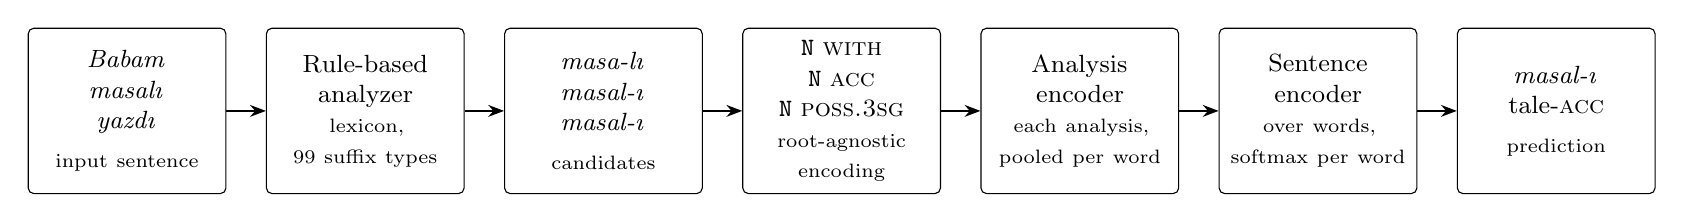
\begin{tikzpicture}[
  node distance=0.5cm,
  box/.style={draw, rounded corners=2pt, align=center, font=\small, minimum height=2.1cm, text width=2.3cm, inner sep=3pt},
  note/.style={font=\scriptsize, text=black!70},
  arr/.style={-{Stealth[length=2mm]}, thick}
]
\node[box] (in) {\tr{Babam}\\ \tr{masalı}\\ \tr{yazdı}\\[3pt] {\scriptsize input sentence}};
\node[box, right=of in] (an) {Rule-based\\ analyzer\\[3pt] {\scriptsize lexicon,\\ 99 suffix types}};
\node[box, right=of an] (cand) {\tr{masa-lı}\\ \tr{masal-ı}\\ \tr{masal-ı}\\[3pt] {\scriptsize candidates}};
\node[box, right=of cand] (enc) {\tok{N} \gl{with}\\ \tok{N} \gl{acc}\\ \tok{N} \gl{poss.3sg}\\[3pt] {\scriptsize root-agnostic\\ encoding}};
\node[box, right=of enc] (tf) {Analysis\\ encoder\\[3pt] {\scriptsize each analysis,\\ pooled per word}};
\node[box, right=of tf] (sent) {Sentence\\ encoder\\[3pt] {\scriptsize over words,\\ softmax per word}};
\node[box, right=of sent] (out) {\tr{masal-ı}\\ tale-\gl{acc}\\[3pt] {\scriptsize prediction}};
\draw[arr] (in) -- (an);
\draw[arr] (an) -- (cand);
\draw[arr] (cand) -- (enc);
\draw[arr] (enc) -- (tf);
\draw[arr] (tf) -- (sent);
\draw[arr] (sent) -- (out);
\end{tikzpicture}}
\caption{The \savyar{} pipeline for the word \tr{masalı} in \tr{Babam masalı yazdı} `My father wrote the tale'. The analyzer proposes three analyses. The ranker sees each as a root token (\tok{N} for any nominal root) followed by suffix tokens. It encodes every analysis, pools the analyses of each word, reads the words of the sentence together and picks the highest-scoring analysis of each word.}
\label{fig:pipeline}
\end{figure*}


\savyar{} has two parts (Figure~\ref{fig:pipeline}). A rule-based analyzer lists the analyses of every word in a sentence. A neural ranker scores sentence candidates built from those analyses, and beam search returns the best one. All knowledge of individual roots sits in the analyzer.

\subsection{Analyzer}
\label{sec:analyzer}

\paragraph{Lexicon.}
The analyzer looks up roots in a lexicon of 22,464 nominal and 1,054 verbal entries taken from \TBD{dictionary source}. A dictionary word that the suffix rules derive from a shorter root by its actual derivation is not an entry: \tr{bulun} `be found' is \tr{bul-un} and \tr{durum} `situation' is \tr{dur-um}. Words that only resemble a derivation remain roots (\tr{dolar} `dollar', \tr{gece} `night'), and so do words formed with a suffix the rules do not model (\tr{satıcı} `seller', \tr{öğretmen} `teacher'). The lexicon was built without consulting any treebank, so test sentences cannot influence which candidates exist.

\paragraph{Suffixes.}
The analyzer has 98 suffix types. Each records the category it attaches to and the category it produces: 40 map nouns to nouns, 33 verbs to nouns, 17 verbs to verbs and 2 nouns to verbs, while 6 attach to either category. Each suffix generates its surface allomorphs from the stem, following vowel harmony, consonant alternation and buffer consonants.

\paragraph{Search.}
Every prefix of a word is tried as a root, both as written and after undoing a stem alternation such as final-consonant voicing (\tr{kitab-ı} from \tr{kitap} `book'). From each root a depth-first search attaches suffixes whose allomorph matches the rest of the word. Suffixes fall into 13 ordered groups, from verb-to-verb derivation through negation, compound verbs, category-changing derivation, converbs, plural, possessive, case, the relative \tr{-ki}, the comitative \tr{-lA}, adverbial suffixes and predicative suffixes to person endings. A suffix may not follow a suffix of a later group. Derivational suffixes may follow each other, and the relative \tr{-ki} restarts the order, which licenses \tr{ev-de-ki-ler-den} house-\gl{loc}-\gl{rel}-\gl{pl}-\gl{abl} `from those in the house'.

\paragraph{Root-dependent rules.}
Because the ranker never sees the root, every rule that depends on it is applied here. Closed lists name the verbs that take the causatives \tr{-Ir} (\tr{geç-ir} `spend (time)') and \tr{-Ar} (\tr{çık-ar} `take out'), the 13 monosyllabic verbs whose aorist is \tr{-Ir} (\tr{gel-ir} `comes'), and the roots that lose their last vowel before a vowel-initial suffix (\tr{ağz-ı} `his or her mouth'). Pronoun restrictions are also enforced here: personal pronouns and the demonstratives \tr{bu} and \tr{şu} take no possessive, so \tr{bizi} is only `us' (\gl{acc}). When no lexicon root yields an analysis, as with many proper nouns and acronyms, the analyzer hypothesises a root from the surface form; the suffixes must still span the rest of the word.

\paragraph{Output.}
Each analysis is a root, the category of the root (noun or verb), a suffix sequence and the resulting category. On the TrMor2018 test words, the analyzer returns \TBD{cand-per-word} analyses per word, \TBD{amb-share}\% of words have more than one, and the gold analysis is among the candidates for \TBD{coverage}\% of words.

\subsection{Root-agnostic encoding}
\label{sec:encoding}

The ranker sees each candidate word as a short token sequence. The first token stands for the root: \tok{N} for any nominal root and \tok{V} for any verbal root, or a token of its own for one of 102 closed-class lexemes such as \tr{ben} `I', \tr{bu} `this', \tr{ve} `and', \tr{için} `for' and the question particle \tr{mI}. One token per suffix follows, identified by the suffix type. Every token carries its suffix group and its position in the word, and the vocabulary has 207 entries: 98 suffixes, 102 lexemes, the two root tokens and five special symbols. A sentence candidate is the concatenation of its word sequences, separated by a word boundary symbol and enclosed in begin and end symbols.

Table~\ref{tab:encoding} shows what this representation keeps and what it discards. The three analyses of \tr{masalı} differ in their suffixes and remain distinct. The pronoun reading of \tr{bana} `to me' stays distinct from a reading built on the noun \tr{ban}, because \tr{ben} has a lexeme token. Analyses that differ only in an open-class root of the same category become identical: \tr{yaz-ın} `your summer' and \tr{yazı-n} `your writing' both encode as \tok{N}~\gl{poss.2sg}, and \tr{dol-ar} `it fills' and \tr{dola-r} `it wraps' both encode as \tok{V}~\gl{aor}. Identical encodings receive identical scores. \TBD{state how ties are counted in evaluation and how often they occur on TrMor2018}.

\begin{table}[t]
\centering
\small
\begin{tabular}{@{}lll@{}}
\toprule
Word & Analysis & Encoding \\
\midrule
\multirow{3}{*}{\tr{masalı}} & \tr{masa-lı} table-\gl{with} & \tok{N} \gl{with} \\
 & \tr{masal-ı} tale-\gl{acc} & \tok{N} \gl{acc} \\
 & \tr{masal-ı} tale-\gl{poss.3sg} & \tok{N} \gl{poss.3sg} \\
\midrule
\multirow{2}{*}{\tr{bana}} & \tr{bana} I-\gl{dat} & \tok{ben} \gl{dat} \\
 & \tr{ban-a} \tr{ban}-\gl{dat} & \tok{N} \gl{dat} \\
\midrule
\multirow{2}{*}{\tr{yazın}} & \tr{yaz-ın} summer-\gl{poss.2sg} & \tok{N} \gl{poss.2sg} \\
 & \tr{yazı-n} writing-\gl{poss.2sg} & \tok{N} \gl{poss.2sg} \\
\bottomrule
\end{tabular}
\caption{Candidate analyses and their encodings. The two analyses of \tr{yazın} shown here receive the same encoding. The analyzer proposes four further analyses of \tr{yazın}, including the imperative \tr{yaz-ın} `write!' (\tok{V}~\gl{imp.2pl}), which the encoding keeps apart.}
\label{tab:encoding}
\end{table}

\subsection{Ranker}
\label{sec:ranker}

Each position of a sentence candidate is represented by the concatenation of four embeddings: the token (384 dimensions), its suffix group (8), its position inside the word (16) and its absolute position in the sequence (384). A two-layer perceptron with a GELU activation projects the 792-dimensional vector to 384 dimensions. A six-layer Transformer encoder \citep{vaswani-etal-2017-attention} with pre-layer normalisation, eight attention heads, a feed-forward width of 1,536 and dropout 0.3 contextualises the positions. The score of a candidate $y$ is
\begin{equation}
s(y) = \mathbf{w}^{\top} \mathrm{LN}\Big(\frac{1}{|y|}\sum_{t=1}^{|y|} \mathbf{h}_t\Big) + b,
\end{equation}
where $\mathbf{h}_t$ are the final hidden states and LN is layer normalisation. Sequences are limited to 512 tokens. The model has about 11.5 million parameters.

\subsection{Training}
\label{sec:training}

\paragraph{Candidate sets.}
A training example is a candidate set: the gold sentence $y^{*}$ and a set of negatives. Each negative copies the gold sentence and replaces the analysis of exactly one ambiguous word with a wrong analysis of the same word. A sentence with $a$ ambiguous words receives
\begin{equation}
k = \max\big(5, \min(16, \lceil 2a \rceil)\big)
\end{equation}
negatives. The words are visited in turn, starting from an offset derived from a hash of the sentence, and each word's candidates are visited from a hashed offset as well. This spreads the negatives over the sentence and over the wrong readings of each word while keeping preprocessing deterministic. Negatives whose encoding equals the gold encoding are discarded. Sentences without an ambiguous word yield no candidate set. When the analyzer cannot reach the gold analysis of a word, the gold suffix sequence is encoded directly and the analyzer is run again with the annotated root to obtain alternatives.

\paragraph{Objective.}
Scores within a candidate set $C$ are turned into a distribution with temperature $\tau = 0.1$:
\begin{equation}
\mathcal{L}_{\text{rank}} = -\log \frac{\exp(s(y^{*})/\tau)}{\sum_{y \in C} \exp(s(y)/\tau)}.
\end{equation}
An auxiliary masked-token objective is computed on the gold sequence. Twenty percent of its root and suffix tokens are selected, at least one per sequence; 80\% of the selected tokens are replaced by a mask symbol, 10\% by a random suffix or lexeme token and 10\% are left unchanged. An output layer tied to the input token embeddings predicts the original tokens. The loss is $\mathcal{L} = \mathcal{L}_{\text{rank}} + 0.2\,\mathcal{L}_{\text{mask}}$.

\paragraph{Optimisation.}
We train with AdamW (learning rate $3\times10^{-4}$, weight decay 0.05), 500 warm-up steps followed by cosine decay to 5\% of the peak rate, gradient clipping at norm 1.0 and mixed precision. Batches are formed under limits on padded tokens and attention cells, which are set from the available GPU memory.

\subsection{Decoding}
\label{sec:decoding}

Decoding proceeds from left to right over the words of a sentence. At word $i$, every partial candidate in the beam is extended with every analysis of word $i$, the extended prefixes are scored with $s$ as if they were complete sentences, and the 50 highest-scoring prefixes are kept. Unambiguous words add a single extension. The output is the highest-scoring complete sentence.

\section{Data}
\label{sec:data}

\begin{table*}[t]
\centering
\small
\begin{tabular}{@{}llrrrr@{}}
\toprule
Treebank & Annotation & Sentences & Words & Suffixed words & Adapted sentences \\
\midrule
BOUN \citep{turk-etal-2022-resources} & Universal Dependencies & 9,761 & 100,916 & 66,698 & 9,687 \\
TWT \citep{kayadelen-etal-2020-gold} & \citet{ozturel-etal-2019-syntactically} features & 4,851 & 57,415 & 40,005 & 4,849 \\
METU-Sabancı \citep{oflazer-etal-2003-building} & inflectional groups & 5,620 & 45,999 & 35,052 & 5,563 \\
TrMor2006 \citep{yuret-ture-2006-learning} & inflectional groups & 50,674 & 729,960 & 497,364 & 47,285 \\
TrMor2018 \citep{akyurek-etal-2019-morphological} & inflectional groups & 34,673 & 388,754 & 280,384 & 33,912 \\
\midrule
Total & & 105,579 & 1,323,044 & 919,503 & 101,296 \\
\bottomrule
\end{tabular}
\caption{Treebanks and the output of the adapters. Words exclude punctuation. Suffixed words have at least one suffix in their gold analysis. Adapted sentences are those that remain after adaptation and after removing sentences that occur in more than one treebank. The METU-Sabancı count includes the 1,000 sentences we hold out as a test set (\S\ref{sec:metu}). The TrMor2018 experiments use all 34,673 TrMor2018 sentences without cross-treebank deduplication.}
\label{tab:corpora}
\end{table*}

We use five Turkish treebanks with three annotation schemes (Table~\ref{tab:corpora}). BOUN \citep{turk-etal-2022-resources} follows Universal Dependencies. The Turkish Web Treebank (TWT; \citealp{kayadelen-etal-2020-gold}) uses the features of the analyzer of \citet{ozturel-etal-2019-syntactically}. METU-Sabancı \citep{oflazer-etal-2003-building}, TrMor2006 \citep{yuret-ture-2006-learning} and TrMor2018 \citep{akyurek-etal-2019-morphological} use the inflectional-group format of \citet{oflazer-1994-two}. TrMor2006 was disambiguated semi-automatically. TrMor2018 was annotated semi-automatically in several passes and disagrees with a hand-tagged subset of 26,819 words in 4.4\% of cases \citep{akyurek-etal-2019-morphological}.

\paragraph{Adapters.}
None of these schemes matches the suffix inventory of \savyar{}, so each treebank has an adapter that maps a gold annotation to a root and a sequence of \savyar{} suffixes. The adapter translates each feature or inflectional group into suffix names, resolves cases where one feature corresponds to several suffix types by comparing with the analyses that the analyzer produces for the word, and drops punctuation. Treebank lemmas that the lexicon treats as derived are expanded through a table of 28,480 dictionary decompositions, so that gold \tr{kullan-ıyor} `uses' becomes \tr{kul-la-n-ıyor}. This table rewrites gold labels only and never adds a candidate. A word whose annotation cannot be mapped marks its sentence as partially trainable; Table~\ref{tab:corpora} reports the sentences that survive.

\paragraph{Splits.}
For the main experiment we follow \citet{akyurek-etal-2019-morphological}, who give TrMor2018 no fixed split and average over five random 80/10/10 splits of its sentences (\S\ref{sec:setup}). The other four treebanks are used only for the secondary evaluation on held-out METU-Sabancı sentences (\S\ref{sec:metu}).

\section{Experimental Setup}
\label{sec:setup}

\paragraph{Protocol.}
We adapt all 34,673 TrMor2018 sentences and split them at random into 80\% training, 10\% development and 10\% test, once for each of the seeds 1 to 5, following \citet{akyurek-etal-2019-morphological}. For every split we train a freshly initialised model on the training part for eight epochs and keep the epoch with the highest accuracy on the ambiguous words of the development part. Each test sentence is processed in one forward pass (\S\ref{sec:ranker}). We report the mean and standard deviation over the five splits. No other treebank is used in these runs.

\paragraph{Scored words.}
\citet{akyurek-etal-2019-morphological} mask digits and proper-noun tags in their evaluation. We exclude digits, \TBD{unanalysed words: confirm definition} and words whose gold annotation the adapter cannot map, together \TBD{5.2}\% of test words. Punctuation is not scored because the adapter removes it.

\paragraph{Metrics.}
A word is correct when the predicted analysis has the gold root and the gold suffix sequence. \TBD{confirm whether the evaluation compares root strings or encodings; this decides how the ties of \S\ref{sec:encoding} count}. We report:
\begin{itemize}
\item word accuracy over all scored words, with words whose gold analysis the analyzer does not propose counted as errors (\emph{uninfused}, following \citealp{seker-tsarfaty-2020-pointer});
\item word accuracy over words whose gold analysis is among the candidates (\emph{infused});
\item accuracy on ambiguous words (more than one candidate) and on unambiguous words;
\item sentence accuracy, the share of sentences in which every scored word is correct;
\item analyzer statistics: coverage of the gold analysis and the number of candidates per word.
\end{itemize}

\paragraph{Comparability.}
Our numbers are not directly comparable with earlier TrMor2018 results for two reasons. First, earlier work counts punctuation tokens, which are unambiguous; TrMor2018 has 460,669 tokens but 388,754 words after adaptation. Second, a \savyar{} analysis is coarser than an analysis in the format of \citet{oflazer-1994-two}: the root category is only noun or verb, so a noun and an adjective with the same suffixes receive the same analysis, and there is no proper-noun feature. Errors of this kind account for a large share of the errors of earlier systems \citep{yildiz-etal-2016-morphology,ozer-korkmaz-2022-transmorph}. The comparison in Table~\ref{tab:comparison} is therefore indicative.

\paragraph{Ablations and diagnostics.}
We compare the full system with the following variants:
\begin{itemize}
\item \emph{Random choice}: the expected accuracy of picking one candidate per word uniformly at random.
\item \emph{Single word}: each word is scored on its own, as a one-word sentence, so the ranker has no context.
\item \emph{No synthetic ambiguity}: the ranker is trained on the real ambiguous words only (\S\ref{sec:training}).
\item \emph{Root-aware}: open-class roots receive their own tokens instead of \tok{N} and \tok{V}. \TBD{describe vocabulary cut-off and training setup}
\item \emph{Gold neighbours}: each ambiguous word is scored with every other word reduced to its gold analysis. This uses gold information and serves as an upper bound on what knowing the analyses of the neighbours could add.
\end{itemize}

\paragraph{Implementation.}
The system is implemented in Python with PyTorch. Each run trains on one NVIDIA GeForce RTX 4050 Laptop GPU with 6\,GB of memory and takes \TBD{train-time} minutes; analysing and disambiguating the test part of one split takes \TBD{decode-time} seconds.

\section{Results}
\label{sec:results}

\begin{table}[t]
\centering
\small
\begin{tabular}{@{}lr@{}}
\toprule
Metric & TrMor2018 (\%) \\
\midrule
All words (uninfused) & 96.16 $\pm$ 0.11 \\
Gold-reachable words (infused) & 96.62 $\pm$ 0.09 \\
Ambiguous words & 92.05 $\pm$ 0.19 \\
Unambiguous words & 99.62 $\pm$ 0.05 \\
Sentences & 68.14 $\pm$ 0.32 \\
\midrule
Gold among candidates & 99.53 \\
Accuracy with punctuation counted & 96.77 $\pm$ 0.09 \\
Ambiguous words (share) & 45.7 \\
Candidates per word & 1.92 \\
Scored words per test split & 37,959 \\
\bottomrule
\end{tabular}
\caption{\savyar{} on TrMor2018: mean and standard deviation over five random 80/10/10 splits. Candidates per word is an average, not a percentage.}
\label{tab:main}
\end{table}

Table~\ref{tab:main} gives the results on TrMor2018. Over all scored words, \savyar{} is correct on 96.16\% of words. On words whose gold analysis the analyzer proposes, accuracy is 96.62\%, so analyzer coverage accounts for 0.46 points of the remaining error. On ambiguous words accuracy is 92.05\%. Unambiguous words are correct exactly when the analyzer's single candidate is the gold one, so their accuracy, 99.62\%, measures coverage on this subset. The standard deviation across splits is at most 0.32 points (Figure~\ref{fig:splits}).

\begin{figure}[t]
\centering
\begin{tikzpicture}
\begin{axis}[
  ybar,
  bar width=7pt,
  width=\columnwidth,
  height=4.6cm,
  xlabel={TrMor2018 split (seed)},
  ylabel={Accuracy (\%)},
  xtick={1,2,3,4,5},
  ymin=80, ymax=100,
  enlarge x limits=0.15,
  ymajorgrids,
  grid style={black!15},
  tick label style={font=\small},
  label style={font=\small},
  legend style={at={(0.5,1.03)}, anchor=south, legend columns=2, draw=none, font=\small},
]
\addplot[fill=black!65, draw=black] table[x=split, y=all, col sep=comma] {data/split_accuracy.csv};
\addplot[fill=black!20, draw=black] table[x=split, y=ambiguous, col sep=comma] {data/split_accuracy.csv};
\legend{All words, Ambiguous words}
\end{axis}
\end{tikzpicture}
\caption{Accuracy of \savyar{} on each TrMor2018 test split.}
\label{fig:splits}
\end{figure}


\begin{table*}[t]
\centering
\footnotesize
\begin{tabular}{@{}lllllr@{}}
\toprule
System & Data & Evaluation & Units & Words scored & Acc. (\%) \\
\midrule
\citet{yuret-ture-2006-learning} & TrMor2006 & hand-tagged test, 862 tokens & lemma + tags & all & 95.82 \\
\citet{sak-etal-2007-morphological} & TrMor2006 & hand-tagged test, 862 tokens & lemma + tags & all & 96.28 \\
\multirow{2}{*}{\citet{shen-etal-2016-role}} & \multirow{2}{*}{TrMor2006} & \multirow{2}{*}{hand-tagged test, 862 tokens} & \multirow{2}{*}{lemma + tags} & all & 96.41 \\
 & & & & ambiguous & 91.03 \\
\citet{yildiz-etal-2016-morphology} & TrMor2016 & re-annotated test, 20K tokens & lemma + tags & ambiguous & 85.18 \\
\multirow{2}{*}{\citet{toleu-etal-2017-character}} & \multirow{2}{*}{TrMor2016} & \multirow{2}{*}{re-annotated test, 20K tokens} & \multirow{2}{*}{lemma + tags} & all & 92.32 \\
 & & & & ambiguous & 84.32 \\
\midrule
\multirow{2}{*}{Morse \citep{akyurek-etal-2019-morphological}} & \multirow{2}{*}{TrMor2018} & \multirow{2}{*}{5 random splits} & \multirow{2}{*}{lemma + tags} & all & 97.67 \\
 & & & & ambiguous & 96.43 \\
MorseDisamb \citep{akyurek-etal-2019-morphological} & TrMor2018 & 5 random splits & lemma + tags & all & 98.59 \\
Transmorph \citep{ozer-korkmaz-2022-transmorph} & TrMor2018 & 10-fold cross-validation & lemma + tags & all & 96.19 \\
\midrule
\multirow{2}{*}{\savyar{}} & \multirow{2}{*}{TrMor2018} & \multirow{2}{*}{5 random splits} & \multirow{2}{*}{root + suffixes} & all & 96.16 \\
 & & & & ambiguous & 92.05 \\
\bottomrule
\end{tabular}
\caption{Published Turkish results and \savyar{}. Rows differ in data, test set, unit of analysis and the tokens that are scored, so only rows on the same data and evaluation are directly comparable. Earlier systems score punctuation tokens; \savyar{} does not. The Morse ambiguous-word figure is from the ablation of \citet{akyurek-etal-2019-morphological}. With proper-noun tags and digits masked, Transmorph reaches about 97\% \citep{ozer-korkmaz-2022-transmorph}.}
\label{tab:comparison}
\end{table*}

Table~\ref{tab:comparison} places these numbers next to published results. The closest comparison is Morse, evaluated under the same protocol: \savyar{} is 1.51 points below Morse on all words and 4.38 points below on ambiguous words. Because \savyar{} predicts a coarser analysis and does not score punctuation (\S\ref{sec:setup}), the difference bounds neither system's accuracy on the other's task.

\section{Analysis}
\label{sec:analysis}

\begin{table}[t]
\centering
\small
\begin{tabular}{@{}lrr@{}}
\toprule
System & All words & Ambiguous \\
\midrule
Random choice (expected) & 72.06 & 39.25 \\
Single word, no context & 94.64 & 88.71 \\
No synthetic ambiguity & 95.96 & 91.60 \\
\savyar{} & \textbf{96.16} & \textbf{92.05} \\
\midrule
Gold neighbours (diagnostic) & --- & 91.90 \\
\bottomrule
\end{tabular}
\caption{Ablations on TrMor2018, mean accuracy (\%) over five splits. The gold-neighbour diagnostic fixes every other word to its gold analysis and is not a valid system; it is measured on ambiguous words only.}
\label{tab:ablation}
\end{table}

\paragraph{Sentence context.}
Scoring each word on its own reaches 88.71\% on ambiguous words, against 92.05\% with the whole sentence (Table~\ref{tab:ablation}). \citet{akyurek-etal-2019-morphological} report a similar comparison for Morse, where context raises ambiguous-token accuracy from 94.38\% to 96.21\%, and in the experiments of \citet{shen-etal-2016-role} full-sentence context raises ambiguous-token accuracy on the hand-tagged TrMor2006 test from 88.65\% to 91.03\%. Figure~\ref{fig:by-candidates} shows that the gain from context grows with the number of candidates, from 2.6 points at two candidates to 9.0 points at six or more. Replacing the neighbours of a word by their gold analyses does not help: accuracy on ambiguous words is then 91.90\%, 0.15 points \emph{below} the full system. Reading every analysis of its neighbours therefore costs the ranker nothing against being told the right one, and the uncertainty of the context is not what limits it.

\begin{figure}[t]
\centering
\begin{tikzpicture}
\begin{axis}[
  width=\columnwidth,
  height=4.6cm,
  xlabel={Candidate analyses per word},
  ylabel={Accuracy (\%)},
  xtick={2,3,4,5,6},
  xticklabels={2,3,4,5,$\geq$6},
  ymin=50, ymax=100,
  ymajorgrids,
  grid style={black!15},
  tick label style={font=\small},
  label style={font=\small},
  legend style={at={(0.03,0.05)}, anchor=south west, draw=none, font=\small},
]
\addplot[mark=*, thick, black] table[x=candidates, y=full, col sep=comma] {data/accuracy_by_candidates.csv};
\addplot[mark=square*, thick, dashed, black!55] table[x=candidates, y=single, col sep=comma] {data/accuracy_by_candidates.csv};
\legend{Sentence context, Single word}
\end{axis}
\end{tikzpicture}
\caption{Accuracy on ambiguous TrMor2018 test words by the number of candidate analyses, pooled over the five splits.}
\label{fig:by-candidates}
\end{figure}


\paragraph{The root abstraction.}
Two measurements bound what the abstraction costs. Analyses that differ only in an open-class root of the same category receive the same score, and the ranker breaks the tie arbitrarily; such ties arise for 1.7\% of ambiguous test words and account for 4.3\% of all errors. Separately, 10.48\% of scored words have a gold analysis that another attested analysis of the same form maps onto, so the coarse label space hides a distinction the annotation makes (\S\ref{sec:limitations-collapse}). We do not report a root-aware ranker: giving open-class roots their own tokens defeats the purpose of the design, and the comparison we would want is against a system that keeps the abstraction but splits the root token by category, which we leave to future work.

\paragraph{Ambiguity profile.}
Figure~\ref{fig:candidates} shows how many analyses the analyzer proposes per word. On the TrMor2018 test words, 54.3\% have a single analysis, 25.5\% have two and 2.3\% have six or more, for an average of 1.92. Earlier work reports 1.60 analyses per token on the TrMor2006 training data for the analyzer of \citet{oflazer-1994-two} \citep{shen-etal-2016-role}. The figures come from different corpora and count different units, so they show only that the two analyzers produce ambiguity of a similar order.

\begin{figure}[t]
\centering
\begin{tikzpicture}
\begin{axis}[
  ybar,
  bar width=6pt,
  width=\columnwidth,
  height=4.4cm,
  xlabel={Candidate analyses per word},
  ylabel={Words (\%)},
  xtick={1,2,3,4,5,6},
  xticklabels={1,2,3,4,5,$\geq$6},
  ymin=0, ymax=60,
  enlarge x limits=0.12,
  ymajorgrids,
  grid style={black!15},
  tick label style={font=\small},
  label style={font=\small},
  legend style={at={(0.97,0.95)}, anchor=north east, draw=none, font=\small},
]
\addplot[fill=black!65, draw=black] table[x=candidates, y=metu, col sep=comma] {data/candidate_distribution.csv};
\addplot[fill=black!20, draw=black] table[x=candidates, y=trmor2018, col sep=comma] {data/candidate_distribution.csv};
\legend{METU-Sabancı test, TrMor2018 test}
\end{axis}
\end{tikzpicture}
\caption{Distribution of the number of analyses the analyzer proposes per word. The METU-Sabancı values are measured on the 9,177 held-out words. \TBD{TrMor2018 values are placeholders: fill the trmor2018 column of data/candidate\_distribution.csv}}
\label{fig:candidates}
\end{figure}


\begin{table}[t]
\centering
\small
\begin{tabular}{@{}llr@{}}
\toprule
Error type & Example & Share (\%) \\
\midrule
Gold not proposed & & 12.4 \\
Accusative vs.\ possessive & \tr{masal-ı} & \TBD{err-acc-poss} \\
Nominal vs.\ verbal root & \tr{dolar}, \tr{dol-ar} & \TBD{err-n-v} \\
Identical encoding & \tr{yaz-ın}, \tr{yazı-n} & 4.3 \\
Other suffix confusion & & \TBD{err-other} \\
\bottomrule
\end{tabular}
\caption{Errors of \savyar{} on TrMor2018, pooled over the five test splits. \TBD{error categories to be revised after inspecting the errors}}
\label{tab:errors}
\end{table}

\paragraph{Errors.}
Table~\ref{tab:errors} groups the errors. 12.4\% of errors are words whose gold analysis the analyzer does not propose; these can only be fixed in the analyzer or the lexicon. The most frequent confusion within the candidate set is \TBD{top-confusion}. \TBD{two or three sentences on characteristic errors, with glossed examples}.

\section{Conclusion}
\label{sec:conclusion}

We presented \savyar{}, a Turkish morphological disambiguator that ranks the output of a rule-based analyzer without seeing open-class roots. Root-specific rules are applied when candidates are generated, and the ranker chooses the suffix sequence of each word in the context of all analyses of the sentence. Because the ranker never sees the root, unambiguous training words can be presented with the analyses of ambiguous words, which adds \TBD{synth-gain} points on ambiguous words. On TrMor2018, under the protocol of \citet{akyurek-etal-2019-morphological}, \savyar{} reaches \TBD{acc-all}\% on all words and \TBD{acc-amb}\% on ambiguous words. The analyzer proposes the gold analysis for \TBD{coverage}\% of words, so \TBD{coverage-share}\% of the remaining errors lie in the analyzer rather than the ranker. Sentence context adds \TBD{context-gain} points on ambiguous words, and giving the ranker access to roots changes accuracy by \TBD{root-delta} points.

Two directions follow from these results. Mapping \savyar{} analyses back to Universal Dependencies features would allow evaluation on the UD Turkish treebanks used in the SIGMORPHON 2019 shared task \citep{mccarthy-etal-2019-sigmorphon} and by \citet{can-etal-2022-joint}. Splitting the root token by finer categories, for example separating adjectives and proper nouns from other nominals, would address the distinctions that the current encoding cannot express. \TBD{revise once the root-aware result is known}.

\section*{Limitations}

\paragraph{Coarse analyses.}
A \savyar{} analysis records only whether a root is nominal or verbal and has no proper-noun feature. It cannot distinguish a noun from an adjective with the same suffixes, which are frequent error types for systems evaluated on the full tag set \citep{yildiz-etal-2016-morphology,ozer-korkmaz-2022-transmorph}. Our accuracy is measured on this coarser representation and is not a measure of accuracy on lemma and full tags.

\paragraph{Dependence on the analyzer.}
The ranker cannot output an analysis that the analyzer does not propose. Coverage depends on a lexicon of 22,464 nominal and 1,054 verbal roots and on 99 suffix types. Words outside the lexicon receive hypothesised roots, which may be wrong even when the suffixes are right.

\paragraph{Identical encodings.}
Analyses that differ only in an open-class root of the same category receive the same score (\S\ref{sec:encoding}). The ranker has no information to choose between them.

\paragraph{Evaluation data.}
TrMor2018 was annotated semi-automatically and disagrees with a hand-tagged subset in 4.4\% of cases \citep{akyurek-etal-2019-morphological}. Our test sets pass through an adapter, and 2.50\% of words are left unscored (\S\ref{sec:setup}). Punctuation is scored but assigned by rule rather than predicted, which credits 15.6\% of the tokens of the corpus without the ranker contributing to them; we therefore report accuracy without punctuation as well.

\paragraph{Collapsed distinctions.}
\label{sec:limitations-collapse}
Our label space is coarser than the TrMor2018 tagset, so some gold distinctions cannot be got wrong. For 10.48\% of the scored words, another analysis attested for the same form maps to the same root and suffix sequence as the gold one, most often a noun read as an adjective or a determiner read as a noun. These words count as correct however the ranker scores them, and no accuracy we report should be read as accuracy on the full TrMor2018 tagset.

\paragraph{Scope.}
We evaluate on Turkish only. Hyperparameters were not tuned beyond a sweep of 23 configurations on the development part of a single split, which varied the learning rate, batch size, dropout, weight decay, width and depth; every configuration except the two largest learning rates fell within a range narrower than the effect of the initialisation seed, so the default configuration was kept. All runs use a single 6\,GB laptop GPU, which limited model size and the number of training epochs.


\bibliography{references}

\end{document}
